\documentclass[12pt]{article}
\usepackage[ruled,vlined]{algorithm2e}
\usepackage{amsmath}
\usepackage{amsfonts}
\usepackage{comment}
\usepackage{enumerate}
\usepackage[top=1in, bottom=1in, left=0.8in, right=1in]{geometry}
\usepackage{listings}
\usepackage{multicol}
\usepackage{hyperref}

\usepackage{tikz}
\usetikzlibrary{positioning}

\usepackage{wrapfig}

\lstset{language=Java, basicstyle={\small\ttfamily}, columns=flexible, belowskip=0mm}
\setlength{\columnsep}{0.1pc}

\begin{document}
\noindent
CS 344 \hfill \textbf{Problem Set 4} \newline 
{Spring 2024} \hfill \textbf{Due:} April 29, 2024, 11:59 p.m.

\noindent
\rule{\linewidth}{0.4pt}
\vspace{.4cm}

\textbf{Name}: ({\color{blue}Replace me with your name})~~~~~\textbf{NetID}: ({\color{blue}Replace me with your NetID})

\vspace{.5cm}

\textbf{Honor Code}: Students may discuss and work on homework problems in groups, which is encouraged. However, each student must write down their solutions independently to show they understand the solution well enough to reconstruct it by themselves.  Students should clearly mention the names of the other students who offered discussions. We check all submissions for plagiarism. We take the honor code seriously and expect students to do the same.


\vspace{.5cm}

\textbf{Instruction for Submission}: This homework has a total of 10 points and 5 bonus points. We encourage you to use LaTex to write your answer, because it's particularly suitable to type equations and it's frequently used for writing academic papers. We have provided the homework3.tex file for you, you can write your answer to each question in this .tex file directly after the corresponding question, and then compile the .tex file into a PDF file for submission. As a quick introduction to LaTex, please see this \textit{Learn LaTeX in 30 minutes} \footnote{\url{https://www.overleaf.com/learn/latex/Learn_LaTeX_in_30_minutes}}. Compiling a .tex file into a PDF file needs installing the LaTex software on your laptop. It's free and open source. But if you don't want to install the software, you can just use this website \url{https://www.overleaf.com/}, which is also free of charge. You can just create an empty project in this website and upload the homework1.zip, and then the website will compile the PDF for you. You can also directly edit your answers on the website and instantly compile your file. You can also use Microsoft Word or other software if you don't want to use LaTex. If so, please clearly number your answers so that we know which answer corresponds to which question. You also need to save your answers as a PDF file for submission. Finally, please submit your PDF file only. You should name your PDF file as ``{\color{blue}{Firstname-Lastname-NetID.pdf'}}'.

\vspace{.5cm}

\textbf{Late Policy}: The homework is due on 4/29 (Monday) at 11:59pm. We will release the solutions of the homework on Canvas on 5/3 (Friday) 11:59pm. If your homework is submitted to Canvas before 4/29 11:59pm, there will no late penalty. If you submit to Canvas after 4/29 11:59pm and before 5/3 11:59pm (i.e., before we release the solution), your score will be penalized by $0.9^k$, where $k$ is the number of days of late submission. For example, if you submitted on 5/2, and your original score is 80, then your final score will be $80*0.9^3=58.32$ for $3$ days of late submission. If you submit to Canvas after 5/3 11:59pm (i.e., after we release the solution), then you will earn no score for the homework.

\vspace{.5cm}

\noindent
\textbf{Drawing graphs:} You might try \texttt{http://madebyevan.com/fsm/} which allows you to draw graphs with your mouse and convert it into \LaTeX  \,code:

\begin{center}
%%%%%%% GENERATED AUTOMATICALLY BY madebyevan.com/fsm/
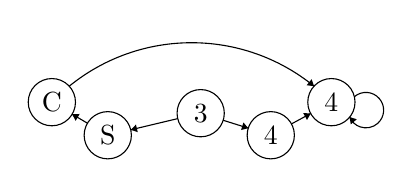
\begin{tikzpicture}[scale=0.1]
\tikzstyle{every node}+=[inner sep=0pt]
\draw [black] (26.7,-13.3) circle (3);
\draw (26.7,-13.3) node {C};
\draw [black] (45.6,-14.7) circle (3);
\draw (45.6,-14.7) node {$3$};
\draw [black] (33.8,-17.5) circle (3);
\draw (33.8,-17.5) node {S};
\draw [black] (54.5,-17.5) circle (3);
\draw (54.5,-17.5) node {$4$};
\draw [black] (62.2,-13.3) circle (3);
\draw (62.2,-13.3) node {$4$};
\draw [black] (42.68,-15.39) -- (36.72,-16.81);
\fill [black] (36.72,-16.81) -- (37.61,-17.11) -- (37.38,-16.14);
\draw [black] (31.22,-15.97) -- (29.28,-14.83);
\fill [black] (29.28,-14.83) -- (29.72,-15.67) -- (30.23,-14.8);
\draw [black] (48.46,-15.6) -- (51.64,-16.6);
\fill [black] (51.64,-16.6) -- (51.03,-15.88) -- (50.73,-16.84);
\draw [black] (57.13,-16.06) -- (59.57,-14.74);
\fill [black] (59.57,-14.74) -- (58.62,-14.68) -- (59.1,-15.56);
\draw [black] (28.907,-11.271) arc (129.11449:50.88551:24.638);
\fill [black] (59.99,-11.27) -- (59.69,-10.38) -- (59.06,-11.15);
\draw [black] (65.108,-12.614) arc (131.00538:-156.99462:2.25);
\fill [black] (64.51,-15.19) -- (64.66,-16.12) -- (65.42,-15.47);
\end{tikzpicture}
\end{center}

You can also draw by hand and insert a picture.

\vspace{.5cm}

\textbf{Make best use of picture in Latex}: If you think some part of your answer is too difficult to type using Latex, you may write that part on paper and scan it as a picture, and then insert that part into Latex as a picture, and finally Latex will compile the picture into the final PDF output. This will make things easier. For instructions of how to insert pictures in Latex, you may refer to the Latex file of our homework 1, which includes several examples of inserting pictures in Latex.


\hrulefill

Discussion Group (People with whom you discussed ideas used in your answers if any):     \\[1ex]


I acknowledge and accept the Honor Code. Please type your initials below:

\textbf{Signed}: ({\color{blue}Replace me with your initials})



\rule{\linewidth}{0.4pt}



\begin{enumerate}

\item \textbf{Longest Common Subsequence} (10 points)

Consider the two sequences \texttt{penguin} and \texttt{chicken}, using the LCS algorithm we learnt in class, find the longest common subsequence of these two words.
\begin{enumerate}
\item (5 points) Work out the 2-dimensional dynamic programming table $T(i,j)$ and provide the length of the LCS. 

\textbf{[You are expected to work out every element of the dynamic programming table.]}

\item (5 points) Traceback on the table to find out the exact longest common subsequence(s) of the two words.

\textbf{[You are required to draw the traceback path(s) on the table and find out all the LCSs.]}
\end{enumerate}

\item \textbf{Longest Increasing Subsequence} (5 bonus points)

Let $A$ be an array of length $n$ containing real numbers.  A \em longest increasing subsequence \em (LIS) of $A$ is a sequence $0 \leq i_1 < i_2 < \ldots i_\ell < n$ so that $A[i_1] < A[i_2] < \cdots < A[i_\ell]$, so that $\ell$ is as long as possible.  For example, if 
$A = [6,3,2,5,6,4,8]$, then an LIS is $i_0 = 2, i_1 = 3, i_2 = 4, i_3 = 6$ corresponding to the subsequence $2,5,6,8$.  (Notice that a longest increasing subsequence does not need to be unique). In the following parts, we will walk through the recipe that we saw in class for coming up with DP algorithms to develop an $O(n^2)$-time algorithm for finding an LIS. 

\begin{enumerate}

\item (2 bonus points) \textbf{(Identify optimal sub-structure and a recursive relationship).}  We will come up with the sub-problems and recursive relationship for you, although you will have to justify it.  Let $D[i]$ be the length of the longest increasing subsequence of $[A[0], \ldots, A[i]]$ that ends on $A[i]$.
Expain why
\[ D[i] = \max_k\{ D[k] + 1\,:\, 0 \leq k < i, A[k] < A[i] \}. \]

[\textbf{Provide a short informal explanation. It is good practice to write a formal proof, but this is not required for credit.}]

\item (2 bonus points) \textbf{(Develop a DP algorithm to find the value of the optimal solution)} Use the relationship above to design a dynamic programming algorithm that returns the \em length \em of the longest increasing subsequence.  Your algorithm should run in time $O(n^2)$ and should fill in the array $D$ defined above.

[\textbf{Provide the pseudo-code, and a brief justification of why the complexity is $O(n^2)$, no formal proof is required.}]

\item (1 bonus points) \textbf{(Adapt the DP algorithm to return the optimal solution)} Adapt your algorithm above by tracking some useful information during the DP procedure, so that it returns the actual LIS, not just its length.

[\textbf{Pseudocode and a short explanation.}]

\textbf{Note:} Actually, there is an $O(n\log n)$-time algorithm to find an LIS, which is faster than the DP solution in this exercise.

\end{enumerate}

\end{enumerate}


\end{document}